\chapter{电势；导体与电容器}\label{ch:b1:potential-capacitors}

场需要三个数来描述每一点；
电势只需一个数。由于静电力是保守力，
电荷分布的全部电场
可以归结为一个标量函数——电势，再通过求导
由它还原出电场，这与力学中由力引出势能所用的
是同一思路。电势就是电压表所示的量，
是电池所维持的量，也是使管中电子加速的量；
它的等势面能一眼看出电场的分布。本章先建立电势的概念，
并以电偶极子（第一个用于描述分子的电模型）为例加以应用，
然后讨论构成每一个电路的两类器件：
导体，其上的电荷自行分布以使内部电场为零；
以及电容器，它在电场中储存电荷和能量。

\begin{omfigure}
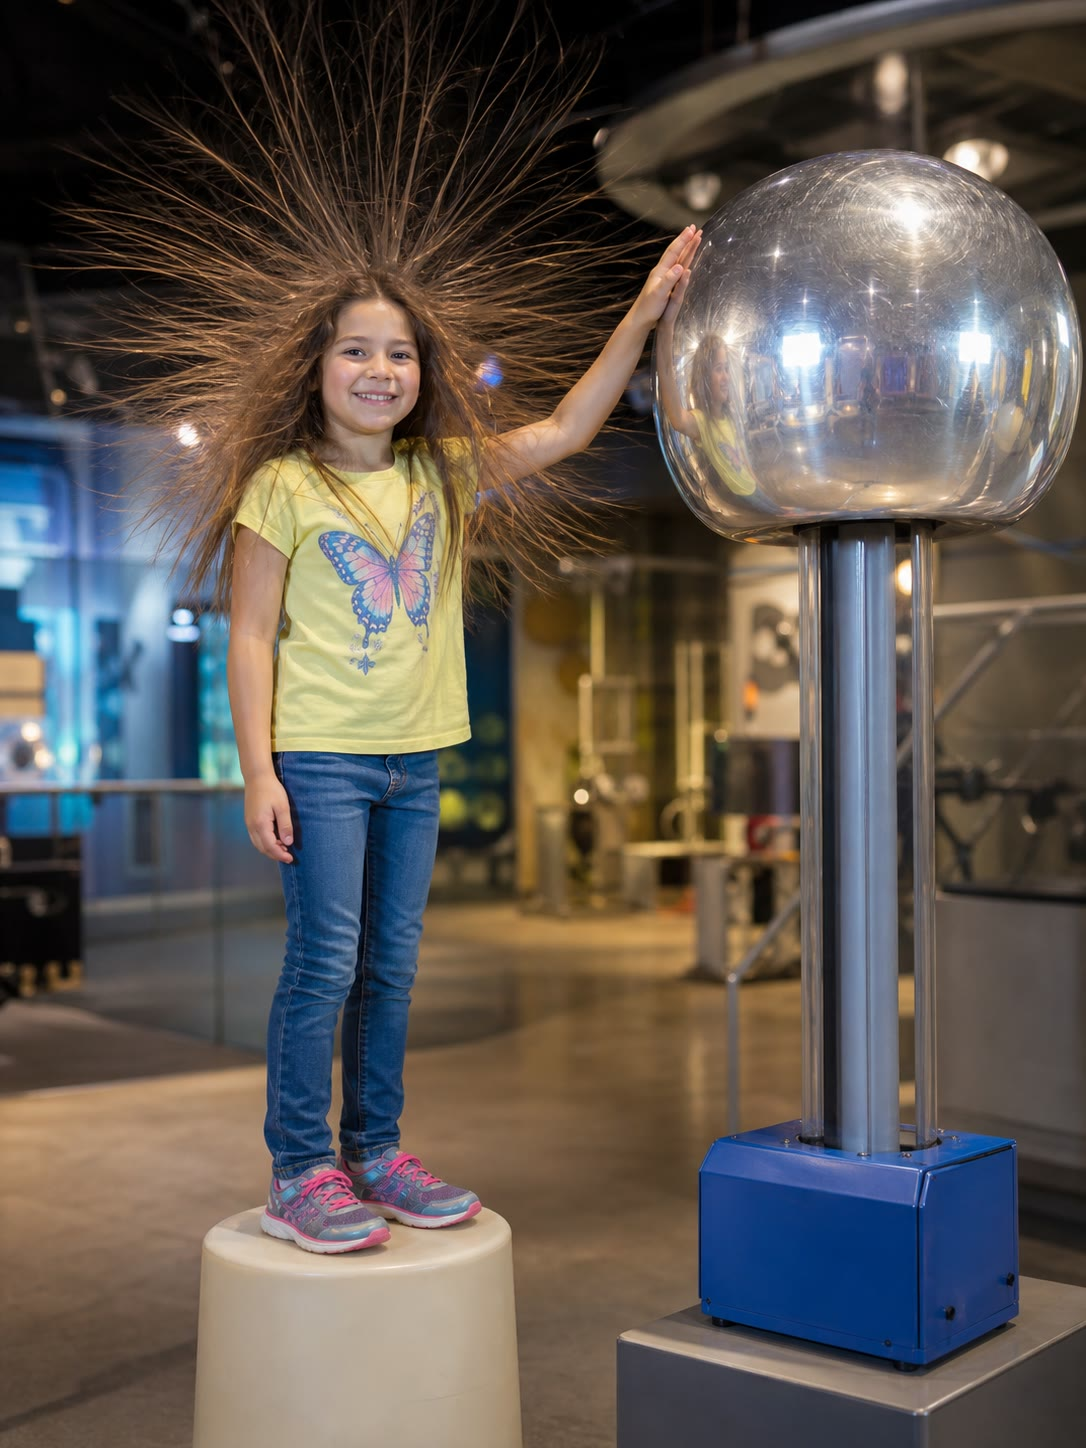
\includegraphics[width=0.34\linewidth]{images/book3/ai/b3-27-van-de-graaff-hair.jpg}

{\small 人体被范德格拉夫起电机充电至数百千伏，成为一个等势导体；身上的头发都处于同一电势、带同种电荷，因而相互排斥。}
\end{omfigure}

\section{静电势}

\begin{theorem}[静电场是保守场]\label{thm:b1:potential-capacitors:potential}
\index{静电势}\index{伏特}\index{环量}
存在一个标量函数 $V(M)$，称为
\emph{静电势}（单位为伏特，\unit{V}），使得
\[
\vect E = -\overrightarrow{\operatorname{grad}}\,V , \qquad
V_A - V_B = \int_A^B \vect E\cdot\dd\vect l
\]
沿从 $A$ 到 $B$ 的任意路径成立（\emph{环量}——
$\vect E$ 从 $A$ 到 $B$ 的积分与路径无关，沿闭合回路的积分为零）。
对于点电荷 $q$ 位于 $O$ 点的情形，$V(M) = \dfrac{q}{4\pi\varepsilon_0\,OM}$；
按约定 $V(\infty) = 0$；对多个点电荷，电势
代数相加。电荷 $q'$ 位于 $M$ 点时的势能为 $E_p = q'V(M)$，且
电场力从 $A$ 移动到 $B$ 所做的功为 $q'(V_A - V_B)$。
\end{theorem}

\begin{proof}
固定电荷 $q$ 对 $q'$ 的库仑力与牛顿
万有引力形式相同，只需将 $-Gm_1m_2$ 换为 $qq'/4\pi\varepsilon_0$；由推导 $E_p = -Gm_1m_2/r$ 的
同一计算（见\cref{prop:b1:work-and-energy:eps}）可得 $E_p = qq'/4\pi\varepsilon_0r$：
两边除以 $q'$ 即得 $V$，并且 $\vect E = \vect F/q' =
-\overrightarrow{\operatorname{grad}}(E_p)/q'$。叠加原理可将结论
推广到任意电荷分布；
环量公式即是沿路径对梯度
积分所给出的定义。
\end{proof}

\begin{proposition}[电势的读法]\label{prop:b1:potential-capacitors:reading}
\index{等势面}
\begin{enumerate}
  \item \emph{等势面} $V = \text{常数}$ 处处与
        电场线垂直，
        且电场指向\emph{电势降低}的方向。
  \item $|\vect E|$ 是沿最陡方向上 $V$ 的变化率：
        等势面密集之处，电场强。
  \item $V$ 只确定到一个加性常数，只有电势
        差（电压）是可测量的。按约定，取地或无穷远处的
        电势为零。
  \item 在以 $O$ 为对称中心的球坐标中，$E_r = -\dd V/
        \dd r$；在平面极坐标 $(r, \theta)$ 中，
        $E_r = -\partial V/\partial r$，$E_\theta = -\dfrac1r\,\partial V/\partial\theta$。
\end{enumerate}
\end{proposition}

\begin{proof}
在等势面上，对面内任一位移有 $\dd V = -\vect E\cdot\dd\vect l = 0$，
故 $\vect E$ 与该面的法线平行；
沿 $\vect E$ 方向移动时，$\dd V = -E\,\dd l < 0$。极坐标分量由
$\dd V = (\partial V/\partial r)\dd r + (\partial V/\partial\theta)\dd\theta$ 与
$\dd\vect l = \dd r\,\vect e_r + r\,\dd\theta\,\vect e_\theta$ 得出。
\end{proof}

\begin{omfigure}
\begin{tikzpicture}[font=\small, x=1cm, y=1cm, >=Stealth]
  \begin{scope}
    \foreach \r in {0.6,0.85,1.2,1.7,2.4} \draw[omProp, thick] (0,0) circle (\r);
    \foreach \a in {0,30,...,330} \draw[omDef, ->] (0.25,0) ++({\a}:0) -- ++({\a}:2.7) ;
    \fill[omThm] (0,0) circle (2.5pt) node[below left, font=\footnotesize] {$q > 0$};
    \node[omProp, font=\footnotesize] at (2.05,2.05) {$V = \text{常数}$};
    \node[font=\footnotesize] at (0,-3.1) {点电荷：球面 $V \propto 1/r$};
  \end{scope}
  \begin{scope}[xshift=8.4cm]
    \draw[omThm, very thick] (-2.2,-2.2) -- (-2.2,2.2) node[above] {$V_1$};
    \draw[omDef, very thick] (2.2,-2.2) -- (2.2,2.2) node[above] {$V_2 < V_1$};
    \foreach \x in {-1.32,-0.44,0.44,1.32} \draw[omProp, thick] (\x,-2.0) -- (\x,2.0);
    \foreach \y in {-1.5,-0.5,0.5,1.5} \draw[omDef, ->] (-2.1,\y) -- (2.0,\y);
    \node[omProp, font=\footnotesize, anchor=west] at (-1.3,2.25) {等势面};
    \node[font=\footnotesize] at (0,-3.1) {平行板电容器：平面，$V$ 随 $x$ 线性变化};
  \end{scope}
\end{tikzpicture}

{\small 点电荷与平行板电容器的
等势面（橙色）和电场线（蓝色）。
电场线与等势面成直角，并由高电势指向低电势；
等势面密集之处，电场强。}
\end{omfigure}

\begin{method}[计算电势]\label{meth:b1:potential-capacitors:compute}
一种方法是对电荷分布求和 $\dd q/4\pi\varepsilon_0r$（要求求和
可以实际完成，且分布为有限的，使 $V(\infty) = 0$ 有意义）；另一种方法是
沿一条便于计算的路径对 $\dd V = -\vect E\cdot\dd\vect l$ 积分，
积分的起点取在 $V$ 已知的某点，电场由
高斯定理求出。对于无限分布（无限长导线、无限大平面），只能用第二种方法，
且 $V$ 的零点必须取在有限远的某一点。
\end{method}

\begin{proposition}[典型分布的电势]\label{prop:b1:potential-capacitors:classic}
\begin{enumerate}
  \item 半径为 $R$、体内带电 $Q$ 的球体：外部 $V(r) = \dfrac{Q}{4\pi\varepsilon_0r}$；
        内部 $V(r) = \dfrac{Q}{4\pi\varepsilon_0}\,\dfrac{3R^2 - r^2}{2R^3}$，
        因此 $V(0) = \tfrac32\,Q/4\pi\varepsilon_0R$。若 $Q$ 分布在表面，
        则内部 $V$ 处处相等，均为 $Q/4\pi\varepsilon_0R$。
  \item 无限长导线，线电荷密度为 $\lambda$：$V(r) = -\dfrac{\lambda}{2\pi\varepsilon_0}\ln\dfrac{r}{r_0}$。
  \item 平行板电容器，极板 1 到极板 2 的电场为 $E$，两板间距为 $d$：
        $V$ 在两板之间线性下降，且 $V_1 - V_2 = Ed$。
\end{enumerate}
\end{proposition}

\begin{proof}
对 $E_r = -\dd V/\dd r$ 积分，所用的场见
\cref{prop:b1:electrostatics-gauss:three}：球体由无穷远向内积分
（在 $R$ 处的连续性确定内部的积分常数）；导线由 $r_0$ 处积分；
电容器则沿间隙积分。
\end{proof}

\begin{omfigure}
\begin{tikzpicture}
\begin{axis}[omaxis, axis x line=bottom, axis y line=left, width=10cm, height=5.8cm,
    xlabel={$r/R$}, ylabel={},
    xlabel style={at={(axis description cs:0.5,-0.1)}, anchor=north},
    xmin=0, xmax=4, ymin=0, ymax=1.7, xtick={1,2,3}, ytick={0.5,1,1.5}, samples=80, clip=false]
  \addplot[omProp, very thick, domain=0:1] {1.5-0.5*x^2};
  \addplot[omProp, very thick, domain=1:4] {1/x};
  \node[omProp, font=\footnotesize, anchor=east] at (axis cs:3.95,1.5) {$V$（单位 $Q/4\pi\varepsilon_0R$）};
  \addplot[omDef, thick, dashed, domain=0:1] {x};
  \addplot[omDef, thick, dashed, domain=1:4] {1/x^2};
  \node[omDef, font=\footnotesize, anchor=east] at (axis cs:3.95,1.27) {$E$（单位 $Q/4\pi\varepsilon_0R^2$）};
  \node[omProp, font=\footnotesize, anchor=west] at (axis cs:0.05,1.58) {$V(0) = \tfrac32\,V(R)$};
\end{axis}
\end{tikzpicture}

{\small 均匀带电球体的电势（实线）与电场（虚线）。
电势连续，斜率也连续；球内电势为抛物线，
此处电场为线性；球外电势为 $1/r$ 形式。电势的
最大值位于球心，该处电场为零——$V$ 的极大值
点是零场点，反之不成立。}
\end{omfigure}

\begin{example}[电子伏特（再谈）]\label{ex:b1:potential-capacitors:eV}
一个电子穿过 \qty{100}{V} 的间隙，获得 $eU = \qty{100}{eV} =
\qty{1.6e-17}{J}$，无论两电极之间的电场形状如何，
电势使路径无关紧要
（见\cref{def:b1:charged-particles:eV}）。一个 \qty{1}{\micro C} 的电荷与另一电荷相距
\qty{1}{m}，此时 $V = \qty{9}{kV}$，两者共储存
\qty{9}{mJ}；金原子核中心的电势为
\qty{24}{MV}（见\cref{exo:b1:potential-capacitors:6}）。
\end{example}

\section{电偶极子}

\begin{definition}[电偶极子]\label{def:b1:potential-capacitors:dipole}
\index{电偶极子}\index{偶极矩}
两个异号电荷 $-q$ 位于 $N$、$+q$ 位于 $P$，相距 $a = NP$，
构成一个\emph{电偶极子}，其\emph{偶极矩}为
$\vect p = q\,\vect{NP}$（\unit{C.m}），方向由 $-$ 指向 $+$。偶极近似
即研究其在距离 $r \gg a$ 处的场。一个分子，若其正、负电荷
中心不重合，便是电偶极子（如水，$p = \qty{6.2e-30}{C.m}$）；
处于电场中的中性原子也会变为电偶极子
（感应偶极子）。
\end{definition}

\begin{proposition}[电偶极子的场]\label{prop:b1:potential-capacitors:dipolefield}
设点 $M$ 满足 $OM = r \gg a$（$O$ 为 $NP$ 的中点），$\theta$ 为
$\vect p$ 与 $\vect{OM}$ 之间的夹角，则
\[
V(M) = \frac{p\cos\theta}{4\pi\varepsilon_0 r^2}, \qquad
E_r = \frac{2p\cos\theta}{4\pi\varepsilon_0r^3}, \qquad
E_\theta = \frac{p\sin\theta}{4\pi\varepsilon_0r^3} .
\]
偶极子的场按 $1/r^3$ 衰减，比点电荷的 $1/r^2$
衰减更快：远处两电荷近乎相互抵消，
剩下的则是两者的间距。
\end{proposition}

\begin{proof}
$V = \dfrac{q}{4\pi\varepsilon_0}\Bigl(\dfrac1{PM} - \dfrac1{NM}\Bigr)$，其中
$PM \approx r - \tfrac a2\cos\theta$ 且 $NM \approx r + \tfrac a2\cos\theta$
（$\pm\tfrac a2$ 在 $\vect{OM}$ 上的投影）；保留到 $a/r$ 的一阶，
由此 $1/PM - 1/NM \approx a\cos\theta/r^2$。于是 $E_r = -\partial V/\partial r$ 且
$E_\theta = -(1/r)\,\partial V/\partial\theta$。
\end{proof}

\begin{omfigure}
\begin{tikzpicture}[font=\small, x=1cm, y=1cm, >=Stealth]
  \begin{scope}[scale=1.3]
    \fill[omDef] (-0.5,0) circle (2.5pt) node[below left, font=\footnotesize] {$-q$};
    \fill[omThm] (0.5,0) circle (2.5pt) node[below right, font=\footnotesize] {$+q$};
    \draw[->, very thick] (-0.5,0) -- (0.5,0); \node[above, font=\footnotesize] at (0,0.05) {$\vect p$};
    \fill (0,0) circle (1pt); \node[below, font=\footnotesize] at (0,-0.05) {$O$};
    \coordinate (M) at (2.6,1.9);
    \fill (M) circle (1.6pt) node[above right, font=\footnotesize] {$M$};
    \draw[dashed] (0,0) -- (M) node[midway, above left, font=\footnotesize] {$r$};
    \draw[dashed] (-0.5,0) -- (M); \draw[dashed] (0.5,0) -- (M);
    \draw (0.9,0) arc[start angle=0, end angle=36, radius=0.9] node[midway, right, font=\footnotesize] {$\theta$};
    \draw[->, omThm, thick] (M) -- ++(36:0.9) node[right, font=\footnotesize] {$E_r$};
    \draw[->, omThm, thick] (M) -- ++(126:0.6) node[above left, font=\footnotesize] {$E_\theta$};
  \end{scope}
  \begin{scope}[xshift=8.6cm, scale=1.0]
    % field lines: circles through the charges (dipole limit: r = K sin^2 theta)
    \foreach \K in {0.8,1.6,2.6} {
      \draw[omDef, thick, domain=3:177, samples=60, smooth] plot ({\K*sin(\x)*sin(\x)*cos(\x)}, {\K*sin(\x)*sin(\x)*sin(\x)});
      \draw[omDef, thick, domain=183:357, samples=60, smooth] plot ({\K*sin(\x)*sin(\x)*cos(\x)}, {\K*sin(\x)*sin(\x)*sin(\x)});
    }
    % equipotentials r = A sqrt(|cos theta|)
    \foreach \A in {0.9,1.5,2.2} {
      \draw[omProp, thick, domain=-88:88, samples=50, smooth] plot ({\A*sqrt(cos(\x))*cos(\x)}, {\A*sqrt(cos(\x))*sin(\x)});
      \draw[omProp, thick, domain=92:268, samples=50, smooth] plot ({\A*sqrt(-cos(\x))*cos(\x)}, {\A*sqrt(-cos(\x))*sin(\x)});
    }
    \draw[->, very thick] (-0.25,0) -- (0.25,0);
    \node[font=\footnotesize, omProp] at (2.95,0.45) {$V > 0$};
    \node[font=\footnotesize, omProp] at (-2.95,0.45) {$V < 0$};
  \end{scope}
\end{tikzpicture}

{\small 左图：偶极近似的几何关系——$M$ 点从
中心 $O$ 处观察，距离为 $r$，所成夹角为 $\theta$（相对 $\vect p$），并标出
径向与横向场分量。右图：场线（蓝色，
$r \propto \sin^2\theta$）与等势线（橙色，$r \propto
\sqrt{|\cos\theta|}$）为指向右方的偶极子的场线与等势线；过 $O$
且垂直于 $\vect p$ 的平面，是等势面 $V = 0$。}
\end{omfigure}

\begin{proposition}[外场中的偶极子]\label{prop:b1:potential-capacitors:dipoleinfield}
\index{电偶极子!力矩}\index{电偶极子!能量}
偶极子 $\vect p$ 处于匀强场 $\vect E$ 中，所受合力为零，
但受力矩 $\vect\Gamma = \vect p\wedge\vect E$，使其趋向与场同向，
并具有势能 $E_p = -\vect p\cdot\vect E$，
在两者同向时最小。非匀强场中，它还会被拉
向场强较大的区域（一维情形下，$F_x = p\,\dd E/\dd x$
对同向排列的偶极子）。
\end{proposition}

\begin{proof}
两力 $\pm q\vect E$ 相互抵消，它们关于 $O$ 点的力矩为 $\vect{OP}\wedge
q\vect E + \vect{ON}\wedge(-q\vect E) = q\vect{NP}\wedge\vect E$。能量：
$qV(P) - qV(N) = -q\,\vect{NP}\cdot\vect E$ 对匀强场成立（因为 $V(P)
- V(N) = -\vect E\cdot\vect{NP}$）。非匀强场中，偶极子沿 $x$ 轴排列：$F_x =
qE(x + a) - qE(x) \approx qa\,\dd E/\dd x$。
\end{proof}

\begin{example}[梳子为何能吸引纸屑]\label{ex:b1:potential-capacitors:comb}
带电梳子产生的场随距离衰减；一小片
纸屑不带电，被场极化（感应出沿 $\vect E$ 方向的偶极子），而
同向偶极子所受的力 $p\,\dd E/\dd x$ 将其拉向
强场区域，即梳子附近。梳子电荷的正负无关紧要；
同一机制也使气球贴在墙上，并使
水流弯曲。对水分子，$pE$ 在 \qty{1}{MV/m} 的场中
为 \qty{6e-24}{J}，仅是 $600$ 分之一的室温热能 $k_BT$：
只有微弱的净取向能在热翻滚中保留下来，
（见\cref{exo:b1:potential-capacitors:7}）。
\end{example}

\section{静电平衡中的导体}

\begin{theorem}[平衡导体的性质]\label{thm:b1:potential-capacitors:conductor}
\index{平衡导体}\index{库仑定理}\index{法拉第笼}
在自由电荷处于静止的导体中：
\begin{enumerate}
  \item 导体内部 $\vect E = \vect 0$，导体为一个
        等势体：$V$ 在其内部和表面上处处相同。
  \item 任何净电荷都分布在表面上，面密度为
        $\sigma$；内部呈电中性。
  \item 紧贴表面外侧，场垂直于表面，且等于
        $\vect E = \dfrac{\sigma}{\varepsilon_0}\,\vect n$（\emph{库仑定理}）。
  \item 导体内部的空腔若不含电荷，则 $\vect E =
        \vect 0$ 且 $V$ 处处均匀，无论外部如何（\emph{法拉第
        笼}）。
\end{enumerate}
\end{theorem}

\begin{proof}
（1）若有电场，则自由电荷会移动，平衡要求 $\vect E =
\vect 0$，因此任意两内点之间 $\dd V = 0$；表面
是其极限。（2）对导体内部任一闭合面应用高斯定理：
通量为零，所包围电荷为零。（3）表面是一个
等势面，故紧贴表面外侧的 $\vect E$ 与之垂直；一个扁柱形
高斯面跨在表面上，仅外侧面有通量 $E\,\dd S$，
（内部 $\vect E = \vect 0$），电荷为 $\sigma\,\dd S$。（4）空腔
壁是等势面；腔内若有电场线，
则须从壁到壁跨越电势降，这在等势面上不可能；
因此既无电场线，亦无电场（在此形式下予以承认）。
\end{proof}

\begin{example}[尖端效应与避雷针]\label{ex:b1:potential-capacitors:point}
\index{尖端效应}
两个半径分别为 $R_1 > R_2$ 的球，相距很远并以导线相连，
它们具有相同的电势 $V = Q_i/4\pi\varepsilon_0R_i$，于是 $\sigma_i = Q_i/4\pi R_i^2 = \varepsilon_0V/R_i$：
曲率半径越\emph{小}，表面
电荷越\emph{大}，场 $\sigma/\varepsilon_0 = V/R$ 也越强。在尖端处，场
强超过空气的击穿值（\qty{3}{MV/m}），远早于其
他任何地方：空气电离，电荷悄然泄漏。避雷针
借助这一\emph{尖端效应}工作——与其说它吸引雷击，
不如说是为雷击提供通路，并在云下
电荷积聚之前将其泄放。
\end{example}

\begin{omfigure}
\begin{tikzpicture}[font=\small, x=1cm, y=1cm, >=Stealth]
  % Faraday cage
  \begin{scope}
    \draw[fill=omExo!20, draw=omExo, thick] (-1.6,-1.3) rectangle (1.6,1.3);
    \draw[fill=white, draw=omExo, thick] (-1.0,-0.75) rectangle (1.0,0.75);
    \foreach \y in {-1.0,-0.5,0,0.5,1.0} \draw[omDef, ->] (-3.0,\y) -- (-1.65,\y);
    \foreach \y in {-1.0,-0.5,0,0.5,1.0} \draw[omDef, ->] (1.65,\y) -- (3.0,\y);
    \foreach \y in {-1.0,-0.5,0,0.5,1.0} {\node[omDef, font=\scriptsize] at (-1.75,\y+0.18) {$-$}; \node[omThm, font=\scriptsize] at (1.75,\y+0.18) {$+$};}
    \node[font=\footnotesize] at (0,0) {$\vect E = \vect 0$};
    \node[font=\footnotesize] at (0,-1.85) {外场中的导体};
  \end{scope}
  % point effect
  \begin{scope}[xshift=8.4cm]
    \draw[fill=omExo!20, draw=omExo, thick] (-1.2,0) circle (1.2);
    \draw[fill=omExo!20, draw=omExo, thick] (0,0.12) -- (2.4,0.0) -- (0,-0.12) -- cycle;
    \draw[omExo, thick] (2.4,0) circle (0.06);
    \foreach \a in {100,135,170,205,240,275} \draw[omDef, ->] (-1.2,0) ++({\a}:1.25) -- ++({\a}:0.5);
    \foreach \a in {-40,-20,0,20,40} \draw[omDef, ->] (2.4,0) ++({\a}:0.1) -- ++({\a}:1.2);
    \node[font=\footnotesize, omDef] at (-1.2,2.0) {$\sigma$ 小，$E$ 弱};
    \node[font=\footnotesize, omDef] at (2.6,1.0) {$\sigma$ 大，$E$ 强};
    \node[font=\footnotesize] at (0.6,-1.85) {各处 $V$ 相同：场 $\propto 1/R$};
  \end{scope}
\end{tikzpicture}

{\small 左图：置于外场中的空心导体——其表面的感应
电荷抵消了内部及空腔中的场（即
法拉第笼）。右图：尖端效应——对单个等势导体，
表面电荷与外场在
曲率最尖锐处最大。}
\end{omfigure}

\section{电容器}

\begin{definition}[电容]\label{def:b1:potential-capacitors:capacitance}
\index{电容}\index{电容器}\index{法拉}
孤立导体处于电势 $V$ 时带有电荷 $Q$
与 $V$ 成正比：$Q = CV$，$C$ 称为\emph{电容}（法拉，
\unit{F}）；对球体有 $C = 4\pi\varepsilon_0R$。\emph{电容器}是一对
导体（\emph{极板}），两者带等量异号电荷 $\pm Q$，并
彼此相对放置，使电场被限制在两者之间；其
电容为 $C = Q/U$，其中 $U = V_1 - V_2$ 为两
极板之间的电压。该符号与电路定律 $i = C\,\dd u/\dd t$ 曾在
\cref{ch:b1:transient-regimes}中出现过。
\end{definition}

\begin{proposition}[三种电容器]\label{prop:b1:potential-capacitors:three}
\index{平板电容器}\index{球形电容器}\index{柱形电容器}
\begin{enumerate}
  \item 平板：面积为 $S$ 的极板，相距 $d \ll \sqrt S$：
        $C = \dfrac{\varepsilon_0S}{d}$。
  \item 球形：半径分别为 $R_1 < R_2$ 的同心球面：
        $C = \dfrac{4\pi\varepsilon_0R_1R_2}{R_2 - R_1}$。
  \item 柱形（同轴），半径为 $a < b$，长度 $L \gg b$：
        $C = \dfrac{2\pi\varepsilon_0L}{\ln(b/a)}$。
\end{enumerate}
在两极板之间填充相对介电常数为 $\varepsilon_r$ 的绝缘体，
使 $C$ 乘以 $\varepsilon_r$（介质分子发生极化，
削弱电场，常见塑料和玻璃的 $\varepsilon_r = 2$ 至 $10$，
水的为 $80$）。
\end{proposition}

\begin{proof}
各种情形下，两极板之间的电场与
\cref{prop:b1:electrostatics-gauss:three}中的相同：$E = \sigma/\varepsilon_0 = Q/\varepsilon_0S$，
$U = Ed$；$E = Q/4\pi\varepsilon_0r^2$，$U = \int_{R_1}^{R_2}E\,\dd r = \dfrac{Q}{4\pi\varepsilon_0}
\Bigl(\dfrac1{R_1} - \dfrac1{R_2}\Bigr)$；$E = Q/2\pi\varepsilon_0Lr$，$U =
\dfrac{Q}{2\pi\varepsilon_0L}\ln\dfrac ba$。以 $Q$ 除以 $U$ 即得。介质
因子予以承认。
\end{proof}

\begin{theorem}[电容器的能量]\label{thm:b1:potential-capacitors:energy}
\index{电容器的能量}\index{电场的能量密度}
电荷量为 $Q$、电压为 $U$ 的电容器储存的能量为
\[
W = \tfrac12 CU^2 = \tfrac12 QU = \frac{Q^2}{2C} ,
\]
即将电荷从一个极板移到另一个极板所需的功，
克服不断增大的电压。对平板电容器，$W = \tfrac12\varepsilon_0E^2
\times Sd$：能量储存于电场中，其密度为 $\tfrac12\varepsilon_0E^2$
每单位体积——这一结论对任意
静电场都成立。
\end{theorem}

\begin{proof}
将 $\dd q$ 从负极板移到正极板，设此时电荷量为
$q$，所需的功为 $\dd W = (q/C)\,\dd q$；从 $0$ 积分到 $Q$。再
代入 $C = \varepsilon_0S/d$ 和 $U = Ed$；一般的能量密度予以承认。
\end{proof}

\begin{example}[三种电容器及其能量]\label{ex:b1:potential-capacitors:energies}
面积为一平方米的一对箔片，相距 \qty{1}{mm}：$C = 8.85 \times 10^{-12}/
10^{-3} = \qty{8.9}{nF}$——法拉是一个非常大的单位。除颤器的
\qty{150}{\micro F}、\qty{2}{kV} 的电容器：能量为 \qty{300}{J}，在毫秒内释放。
\qty{3000}{F}、\qty{2.7}{V} 的超级电容器，在
一个与汽水瓶同样大小的罐中可储存 \qty{11}{kJ} 能量——其电容来自
极小的分子间隙 $d$ 与极大的多孔面积 $S$。空气击穿时电场的能量密度
为 $\tfrac12\varepsilon_0(3 \times 10^6)^2 = \qty{40}{J/m^3}$，这正是
电容器比电池储存能量少得多的原因。
\end{example}

\begin{omfigure}
\begin{tikzpicture}[font=\small, x=1cm, y=1cm, >=Stealth]
  \begin{scope}
    \draw[omThm, very thick] (-1.5,1) -- (1.5,1) node[right, font=\footnotesize] {$+Q$, $V_1$};
    \draw[omDef, very thick] (-1.5,-1) -- (1.5,-1) node[right, font=\footnotesize] {$-Q$, $V_2$};
    \foreach \x in {-1.1,-0.55,0,0.55,1.1} \draw[omProp, ->] (\x,0.9) -- (\x,-0.85);
    \draw[omProp, dashed] (-1.55,0.9) .. controls (-2.2,0.5) and (-2.2,-0.5) .. (-1.55,-0.85);
    \draw[omProp, dashed] (1.55,0.9) .. controls (2.2,0.5) and (2.2,-0.5) .. (1.55,-0.85);
    \draw[<->] (-2.6,1) -- (-2.6,-1) node[midway, left, font=\footnotesize] {$d$};
    \node[font=\footnotesize] at (0,-1.7) {平板：$C = \varepsilon_0S/d$};
    \node[font=\footnotesize, omProp, fill=white, inner sep=1.5pt] at (0.27,0.3) {$E = U/d$};
  \end{scope}
  \begin{scope}[xshift=6.2cm]
    \draw[omDef, very thick] (0,0) circle (1.3);
    \draw[omThm, very thick, fill=omThm!15] (0,0) circle (0.55);
    \foreach \a in {0,60,...,300} \draw[omProp, ->] (0,0) ++({\a}:0.6) -- ++({\a}:0.6);
    \draw[<->] (0,0) -- (225:0.55) node[midway, above left, font=\scriptsize] {$R_1$};
    \draw[<->] (0,0) -- (-20:1.3) node[pos=0.75, below, font=\scriptsize] {$R_2$};
    \node[font=\footnotesize] at (0,-1.7) {球形（柱形见正文）};
  \end{scope}
  \begin{scope}[xshift=11.2cm]
    \fill[omExo!25] (-1.2,-0.95) rectangle (1.2,0.95);
    \draw[omThm, very thick] (-1.2,1) -- (1.2,1);
    \draw[omDef, very thick] (-1.2,-1) -- (1.2,-1);
    \node[font=\footnotesize] at (0,0) {$\varepsilon_r$};
    \node[font=\footnotesize] at (0,-1.7) {介质填充：$C \to \varepsilon_rC$};
  \end{scope}
\end{tikzpicture}

{\small 平板、球形及介质填充电容器。电场
（橙色）被限制在两极板之间，仅在边缘处有边缘效应，
当 $d$ 很小时可忽略；能量 $\tfrac12\varepsilon_0E^2$
为每单位体积的能量，储存于该电场中。}
\end{omfigure}

\begin{remark}[电容器的组合]\label{rem:b1:potential-capacitors:association}
并联（电压 $U$ 相同）时电荷相加：$C = C_1 + C_2$；串联
（电荷 $Q$ 相同）时电压相加：$1/C = 1/C_1 + 1/C_2$——与
电阻相反，因为 $C$ 衡量的是容易程度（每伏所储电荷），而 $R$
衡量的是困难程度。这些规律由 $Q = CU$ 以及
\cref{ch:b1:dc-circuits}中的电路定律推出。
\end{remark}

\section{练习}

\begin{exercise}[$\star$]\label{exo:b1:potential-capacitors:1}
求距 \qty{1.0}{\micro C} 电荷 \qty{1.0}{m} 处的电势；求将另一个
\qty{1.0}{\micro C} 的电荷由无穷远处移至该点所需的能量；
若其质量为 \qty{1}{g} 且被释放，求它飞离时的速率。
\end{exercise}

\begin{exercise}[$\star$]\label{exo:b1:potential-capacitors:2}
两极板相距 \qty{1.0}{mm}，电压为 \qty{100}{V}：求电场；求
电子从静止穿过间隙时获得的动能和速率；
求飞行时间。
\end{exercise}

\begin{exercise}[$\star$]\label{exo:b1:potential-capacitors:3}
在一张相邻等势线相差 \qty{10}{V} 的图上，
在 $A$ 附近等势线相距 \qty{2}{mm}，在 $B$ 附近相距 \qty{8}{mm}。求 $A$ 点的电场；
与 $B$ 点的电场；电场方向相对于电势增加的方向如何；
电子向哪个方向加速？
\end{exercise}

\begin{exercise}[$\star$]\label{exo:b1:potential-capacitors:4}
一个半径为 \qty{15}{cm} 的范德格拉夫起电球，充电至 \qty{200}{kV}。
求其电容、电荷量及表面的电场。
求其周围空气被击穿前的最大电势（击穿场强为 \qty{3}{MV/m}）。
\end{exercise}

\begin{exercise}[$\star\star$]\label{exo:b1:potential-capacitors:5}
求半径为 $R$、电荷量为 $Q$ 的圆环轴线上的电势；
通过求导得出轴向电场。对均匀带电圆盘做同样的计算
（利用\cref{exo:b1:electrostatics-gauss:5}）：$V(z) = \dfrac{\sigma}{2\varepsilon_0}
\bigl(\sqrt{z^2 + R^2} - z\bigr)$.
\end{exercise}

\begin{exercise}[$\star\star$]\label{exo:b1:potential-capacitors:6}
由均匀带电球体的电场求其内部的电势。
求金原子核（$Z = 79$，$R = \qty{7.0}{fm}$）中心处的电势；
质子从远处抵达中心所需的能量，
以 \unit{MeV} 表示；评论卢瑟福所用的 \qty{5}{MeV} α 粒子。
\end{exercise}

\begin{exercise}[$\star\star$]\label{exo:b1:potential-capacitors:7}
水分子 $p = \qty{6.2e-30}{C.m}$。求其在距离 \qty{1.0}{nm} 处
沿其轴线方向及垂直于轴线方向产生的电场；
求在 $E = \qty{1.0}{MV/m}$ 的电场中，顺向与反向取向之间的力矩及能量差；
并与 \qty{300}{K} 时的 $k_BT$ 作比较。求钠离子
在 \qty{0.3}{nm} 处产生的电场，以及水分子偶极子在其中沿电场取向时的能量（水合作用）。
\end{exercise}

\begin{exercise}[$\star\star$]\label{exo:b1:potential-capacitors:8}
空气中半径为 \qty{1.0}{cm} 的导体球：求其击穿前的最大电荷量，
以及最大电势。两个导体球 $R_1 = \qty{10}{cm}$
与 $R_2 = \qty{1.0}{mm}$ 由细导线相连，并充电至
\qty{20}{kV}：求每个球表面的电场；哪一个球会向空气放电？
\end{exercise}

\begin{exercise}[$\star\star$]\label{exo:b1:potential-capacitors:9}
电容：两块面积为 \qty{1.0}{m^2} 的金属箔相距 \qty{10}{\micro m}，两者之间
填充相对介电常数 $\varepsilon_r = 2.2$ 的聚合物薄膜（薄膜电容器）；将同样的金属箔
卷成圆筒，是否改变 $C$？求其在 \qty{400}{V} 时的能量。一个 \qty{150}{\micro F} 的
电容器充电至 \qty{2.0}{kV}（除颤器）：求其电荷量、能量，以及
若在 \qty{5}{ms} 内放电时的平均功率。
\end{exercise}

\begin{exercise}[$\star\star\star$]\label{exo:b1:potential-capacitors:10}
\emph{球形与柱形电容器。}（a）求同心球的 $C$，
并验证当 $R_2 - R_1 = d \ll R_1$ 时，它化为平行板公式，
当 $R_2 \to \infty$ 时化为孤立球的结果。
（b）同轴电缆，$a = \qty{0.5}{mm}$，$b = \qty{2.5}{mm}$，填充聚乙烯
$\varepsilon_r = 2.3$：求每米电容（与标准电缆的 \qty{100}{pF/m}
作比较）。（c）求内导体处的电场，
在 \qty{1}{kV} 电压下是否安全？
\end{exercise}

\begin{exercise}[$\star\star\star$]\label{exo:b1:potential-capacitors:11}
\emph{场中的能量。}（a）求带电导体球
（$Q$，$R$）的能量，由 $Q^2/2C$ 得出。（b）令其等于电子的静止能量
$m_ec^2 = \qty{0.511}{MeV}$，解出 $R$：即“经典电子
半径”（精确到一个因子）。（c）一个孤立的平行板电容器，带电量为
$Q$，将其极板由 $d$ 拉至 $2d$：求储存能量的变化，并
由此推出极板间的作用力；与
\cref{exo:b1:electrostatics-gauss:8}作比较。（d）同样地，若由电池使电容器保持
$U$ 不变，求能量变化，并说明差值去向何处。
\end{exercise}

\begin{exercise}[$\star\star\star$]\label{exo:b1:potential-capacitors:12}
\emph{原子核的库仑能。}（a）将一个均匀带电
球（$Q$，$R$）逐层叠加，并证明其静电能为
$W = \dfrac{3Q^2}{20\pi\varepsilon_0R}$。（b）铀-238：$Z = 92$，$R =
\qty{7.4}{fm}$：求 $W$，以 \unit{MeV} 表示。（c）将其分裂为两个相等的碎片
（$Z/2$，$A/2$，半径 $R/2^{1/3}$），相距甚远：求释放的库仑能。
（d）实测的裂变能约为 \qty{200}{MeV}：是什么
与库仑能的增益相抗衡？
\end{exercise}

\begin{omfigure}
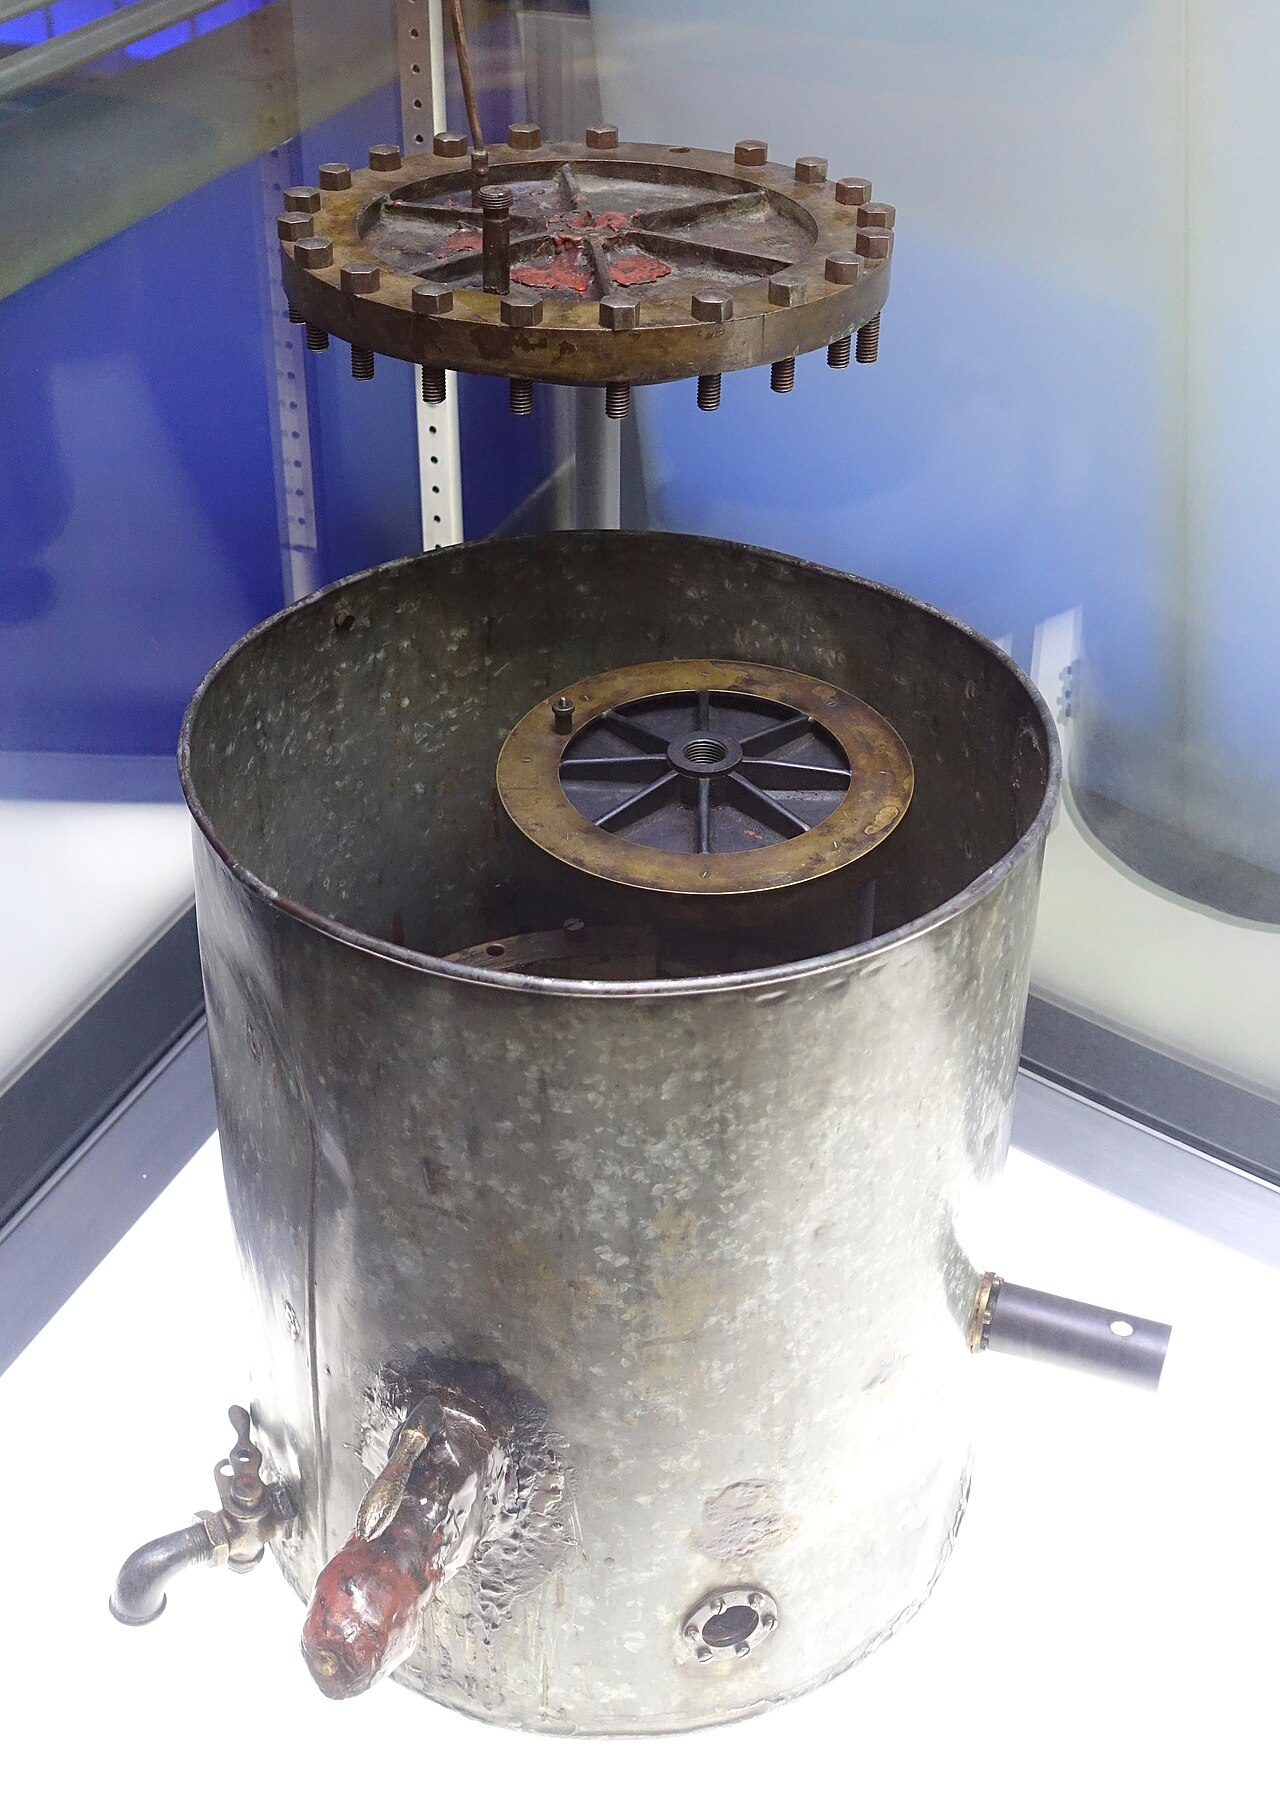
\includegraphics[width=0.36\linewidth]{images/book3/millikan-apparatus.jpg}

{\small 密立根油滴装置，约 1916 年（芝加哥科学与工业博物馆）：黄铜室内装有两块水平极板，油滴在其间被观察。}
\end{omfigure}

\section{问题：密立根油滴}

\begin{problem}[{周末问题——用一滴油称量电子的电荷：
斯托克斯、平行板电容器，以及一张数据表，
其数值只能是元电荷的整数倍}]
\label{pb:b1:potential-capacitors:1}
将油滴喷入两块水平极板之间，两板相距 $d = \qty{16}{mm}$，
极板直径为 \qty{20}{cm}，油滴通过显微镜被观察。
已知：油的密度 $\rho = \qty{900}{kg/m^3}$，空气密度
\qty{1.2}{kg/m^3}，空气黏度 $\eta = \qty{1.8e-5}{Pa.s}$，$g =
\qty{9.8}{m/s^2}$，$\varepsilon_0 = \qty{8.85e-12}{F/m}$。一个在空气中运动的小球，
半径为 $r$、速度为 $v$ 时受到斯托克斯阻力 $6\pi\eta rv$。

\medskip
\noindent\textbf{第一部分——下落的油滴。}
\begin{enumerate}
  \item 未加电压时，下落油滴所受的力；证明其趋于
        终端速度 $v_1 = 2\rho gr^2/9\eta$（忽略空气浮力，并
        说明理由）。
  \item 一滴油在 \qty{10}{s} 内下落 \qty{1.0}{mm}：求其半径和质量。
  \item 趋近 $v_1$ 的时间常数；
        这段时间内下落的距离。油滴是否曾被观察到加速运动？
  \item 运动的雷诺数 $\rho_{\text{空气}}v_1r/\eta$：
        斯托克斯定律是否成立？
  \item 为何油滴必须如此之小？（将其重力与
        一个元电荷在
        \qty{3e5}{V/m} 的电场中所受的电场力作比较。）
  \item 观察到油滴在其平均下落路径附近有轻微抖动：这是什么现象，
        它为何限制了测量精度？
\end{enumerate}

\medskip
\noindent\textbf{第二部分——电场。}
设两极板间加电压 $U$，上极板为正。
\begin{enumerate}[resume]
  \item 求 $U = \qty{5.0}{kV}$ 时两极板间的电场；
        说明其为何是均匀的，并求等势面。
  \item 求两极板的电容，\qty{5.0}{kV} 时极板上的电荷，以及
        储存的能量。
  \item 问题~2 中的油滴在 $U_0 = \qty{1080}{V}$ 时保持静止：
        求其电荷的符号和数值，分别以库仑及 $e$ 为单位。
  \item 当 $U = \qty{5.0}{kV}$ 时，同一油滴以 $v_2$ 上升：证明
        $q = 6\pi\eta r(v_1 + v_2)d/U$，并计算 $v_2$。
  \item 为何测量上升与下落的时间，
        比寻找平衡电压更好？
  \item 求两极板间油滴电荷在
        \qty{5}{kV} 时的势能，以及油滴上升
        \qty{1}{cm} 过程中阻力耗散的能量。
\end{enumerate}

\medskip
\noindent\textbf{第三部分——电荷表。}
在两次测量之间，将同一油滴置于弱 X 射线源中照射，
其电荷随之改变；连续测量所得（单位 $10^{-19}$~C）：
$4.80$, $8.01$, $6.42$, $3.19$, $9.63$.
\begin{enumerate}[resume]
  \item 证明这五个值都接近某一量的整数倍，
        并给出各整数。
  \item 由这五个值给出元电荷的最佳估计值；
        平均值的标准不确定度（见\cref{ch:b1:units-dimensions}）。
  \item 为何两次测量之间电荷的变化
        都是 $e$ 的整数倍？
  \item 证明在此方法中 $q \propto \eta^{3/2}$：黏度有 $1\%$ 的误差时，
        $e$ 会偏移多少？（密立根最初的
        值偏低 $0.6\%$，正是由于此原因。）
  \item 夸克带有 $\pm e/3$ 和 $\pm 2e/3$ 的电荷：为何从未有油滴
        显示出 $e$ 的三分之一？
  \item 法拉第常数，即一摩尔电子所带的电荷，为
        $F = \qty{96485}{C/mol}$：由此推出阿伏伽德罗常数。
  \item 汤姆孙曾测得电子的 $e/m_e = \qty{1.76e11}{C/kg}$：
        求其质量，并与氢原子
        （\qty{1.67e-27}{kg}）作比较。
\end{enumerate}

\medskip
\noindent\textbf{第四部分——从电势看仪器。}
\begin{enumerate}[resume]
  \item 画出两极板间的等势面与电场线，
        包括边缘附近的边缘效应；说明忽略它的理由。
  \item 一带正电的油滴位于下极板上方高度 $z$ 处，
        （下极板电势为 \qty{0}{V}）：求其势能关于 $z$ 的函数；
        计入重力后的总势能；
        以及静止点处 $U$ 应满足的条件。
  \item 将油滴电荷的能量（问题~12）与
        电容器储存的能量作比较：油滴是否扰动了电场？
  \item 将电压反向（下极板为正），
        $U = \qty{5.0}{kV}$：问题~9 中的油滴会如何运动，
        速率为多少？
  \item 一粒质量为 \qty{1}{\micro g} 的尘埃颗粒，在同一电场中带有 $10^4e$ 的电荷：
        求其电场力与重力之比；说明此类颗粒为何无法被悬浮，
        以及密立根为何选用油雾。
  \item 总结：测量了什么（三次），推出了什么，
        带有怎样的不确定度，并由此得出了哪两个常数。
\end{enumerate}
\end{problem}
